\documentclass[12pt,a4paper]{article}
\usepackage{fontspec}
\setmainfont{DejaVu Serif}
\usepackage[margin=2cm]{geometry}
\usepackage{graphicx}
\usepackage{float}
\usepackage{hyperref}
\usepackage{enumitem}
\usepackage{pdflscape}
\usepackage{listings}
\lstset{language=Java,basicstyle=\ttfamily\scriptsize,breaklines=true,frame=single,columns=fullflexible}
\hypersetup{colorlinks=true,urlcolor=blue}
\title{Devoir n°1 : Patrons de construction (INF461)}
\author{KOA ESSAMA PAULIN BRICE\\Matricule : 25I2255}
\date{}
\begin{document}
\maketitle

\section*{Introduction}
Ce rapport présente deux exemples personnels inspirés des formes \textit{Factory Method} et \textit{Factory}. Le premier gère des documents administratifs ; le second gère des moyens de transport. Chaque exemple commence avec trois classes concrètes, puis est modifié par l'ajout d'une quatrième classe.

\section{Exemples personnels initiaux : trois classes concrètes}
Dans les deux cas, le client ne connaît le type concret à utiliser qu'à l'exécution.

\subsection{Factory Method}
Une seule classe \texttt{FabriqueDocument} reçoit le type souhaité et crée une \texttt{AttestationScolarite}, un \texttt{CertificatStage} ou un \texttt{ReleveNotes}. Le client dépend de l'interface \texttt{Document}.
\begin{figure}[H]\centering
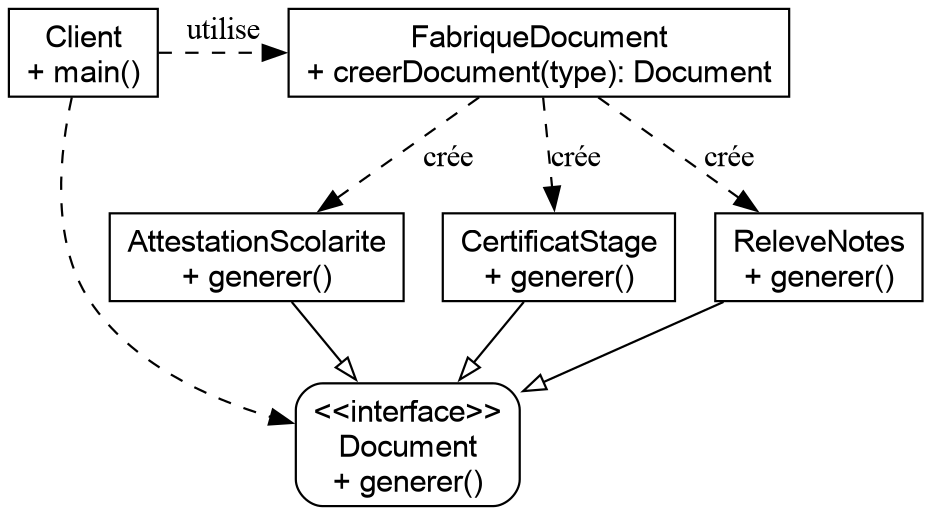
\includegraphics[width=\textwidth,height=.55\textheight,keepaspectratio]{diagrammes/documents_3.png}
\caption{Factory Method -- documents administratifs (3 documents)}
\end{figure}

\subsection{Factory}
\texttt{FabriqueTransport} définit la méthode de création. Les fabriques concrètes créent une \texttt{MotoTaxi}, un \texttt{TaxiVille} ou un \texttt{BusUrbain}.
\begin{figure}[H]\centering
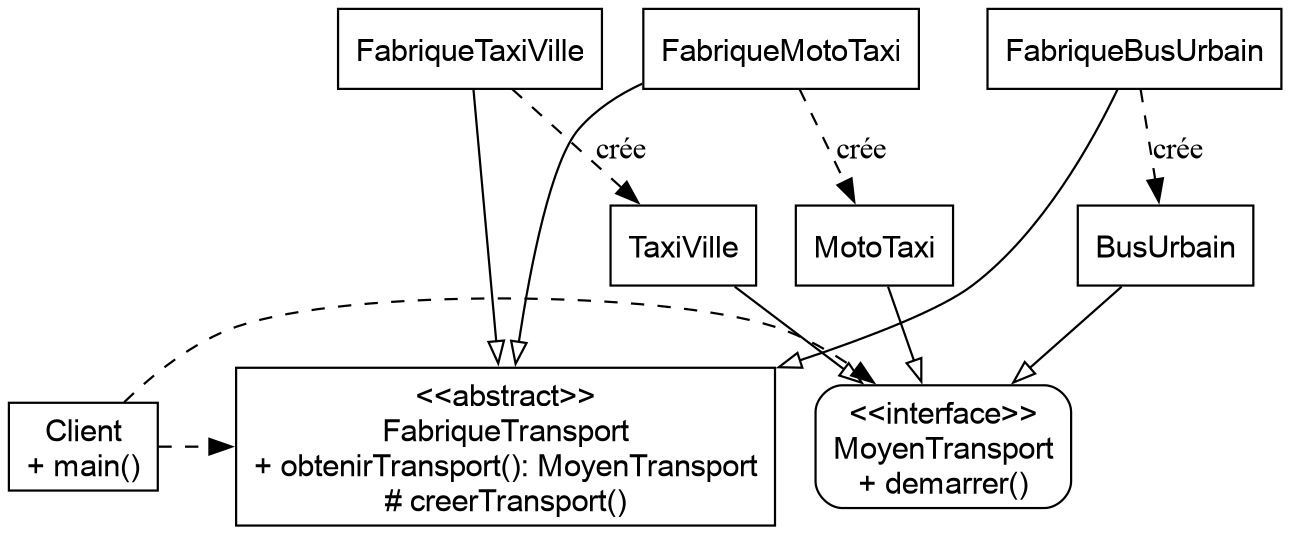
\includegraphics[width=\textwidth,height=.55\textheight,keepaspectratio]{diagrammes/transports_3.png}
\caption{Factory -- moyens de transport (3 transports)}
\end{figure}

\section{Exemple modifié : quatre produits}
La variante ajoute un quatrième élément à chacun des exemples.

\subsection{Factory Method modifié}
On ajoute \texttt{LettreRecommandation} et le cas \texttt{recommandation} dans \texttt{FabriqueDocument}. La fabrique centrale doit donc être modifiée.
\begin{figure}[H]\centering
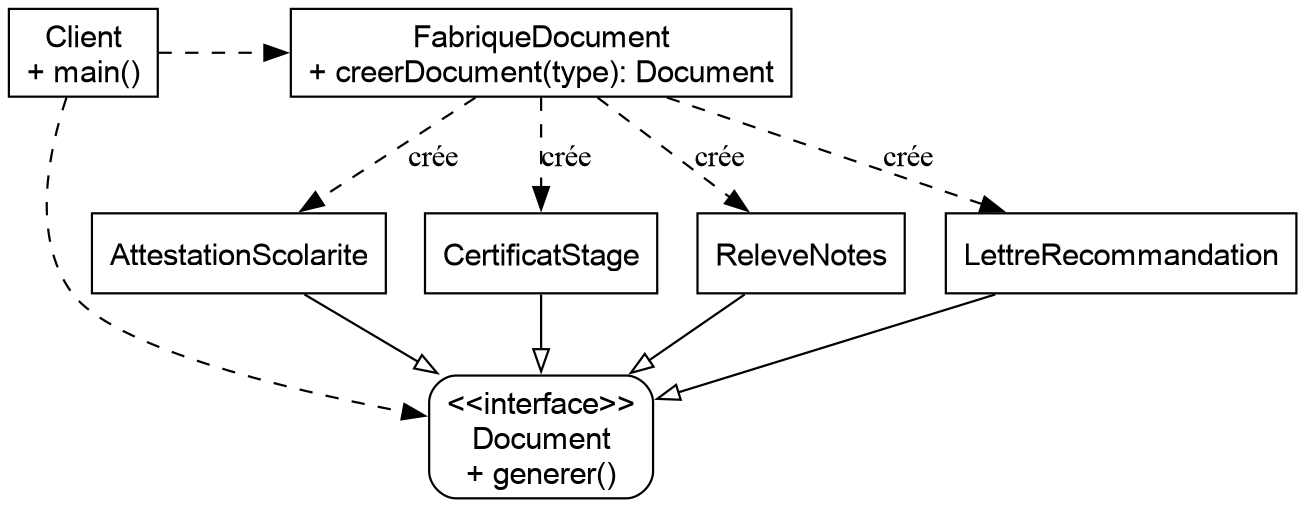
\includegraphics[width=\textwidth,height=.55\textheight,keepaspectratio]{diagrammes/documents_4.png}
\caption{Factory Method -- documents administratifs (4 documents)}
\end{figure}

\subsection{Factory modifié}
On ajoute \texttt{TrainInterurbain} et \texttt{FabriqueTrainInterurbain}. Les classes déjà présentes ne changent pas ; le client peut utiliser la nouvelle fabrique.
\begin{figure}[H]\centering
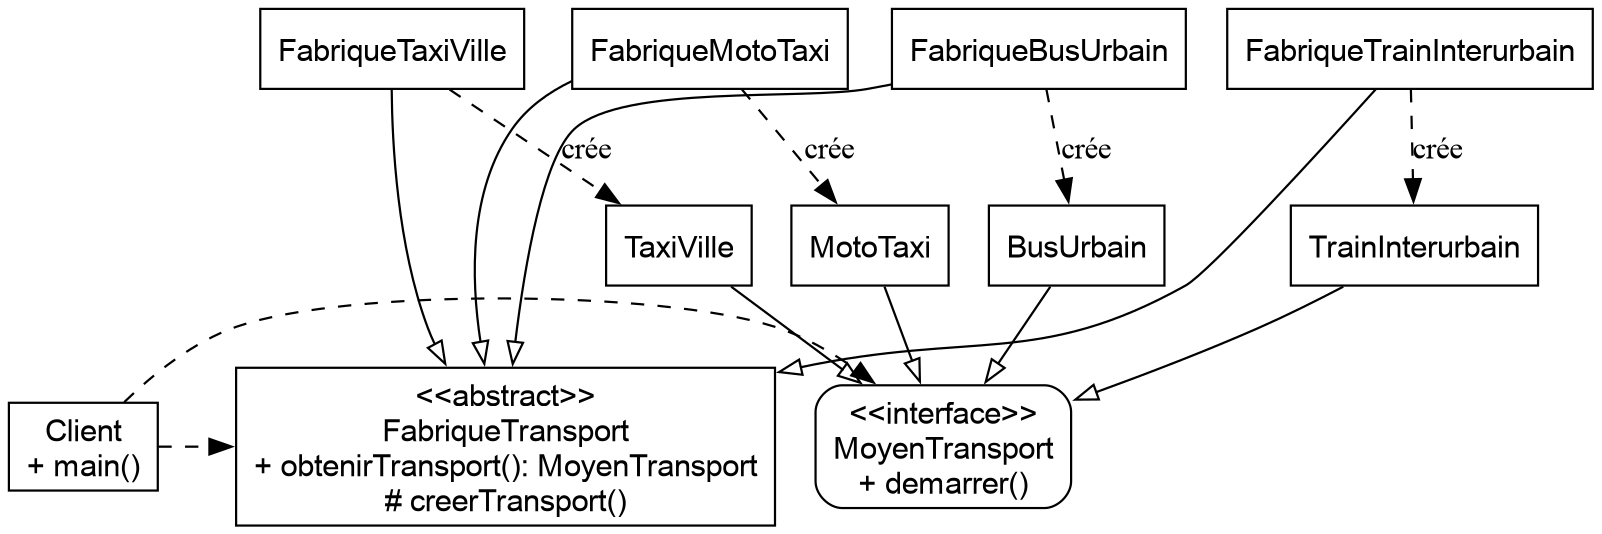
\includegraphics[width=\textwidth,height=.55\textheight,keepaspectratio]{diagrammes/transports_4.png}
\caption{Factory -- moyens de transport (4 transports)}
\end{figure}

\section{Implémentation complète}
Les quatre codes sources sont inclus ci-dessous. Ils peuvent être compilés directement avec Java.
\subsection{Factory Method : documents administratifs (3 documents)}
\lstinputlisting{src/factorymethod/troisproduits/Client.java}

\subsection{Factory Method : documents administratifs (4 documents)}
\lstinputlisting{src/factorymethod/quatreproduits/Client.java}

\subsection{Factory : moyens de transport (3 transports)}
\lstinputlisting{src/factory/troisproduits/Client.java}

\subsection{Factory : moyens de transport (4 transports)}
\lstinputlisting{src/factory/quatreproduits/Client.java}

\section{Organisation du code et dépôt GitHub}
Le code est organisé en quatre packages :
\begin{itemize}[noitemsep]
  \item \texttt{factorymethod.troisproduits} : exemple du cours ;
  \item \texttt{factorymethod.quatreproduits} : variante à quatre produits ;
  \item \texttt{factory.troisproduits} : exemple du cours ;
  \item \texttt{factory.quatreproduits} : variante à quatre produits.
\end{itemize}
Le dépôt public est disponible à l'adresse : \url{https://github.com/eliote-geeks/devoir-inf461-patrons-construction-koa-essama-paulin-brice}.

\section{Analyse des modèles génériques}
\textbf{Factory Method.} Une seule fabrique choisit le document à l'aide d'un paramètre. Cette solution est simple lorsque le type est connu seulement à l'exécution. L'ajout de \texttt{LettreRecommandation} impose toutefois de modifier \texttt{FabriqueDocument}.

\textbf{Factory.} Une fabrique abstraite déclare \texttt{creerTransport()} et chaque sous-classe crée un moyen de transport concret. L'ajout du train consiste à créer \texttt{TrainInterurbain} et \texttt{FabriqueTrainInterurbain}, sans modifier les fabriques existantes. Cette solution respecte mieux le principe ouvert/fermé, mais nécessite davantage de classes.

\section{Modèles génériques}
Les deux modèles génériques étudiés servent de base aux exemples personnels précédents.
\begin{figure}[H]\centering
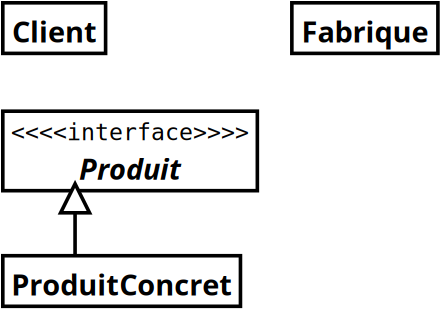
\includegraphics[width=.65\textwidth]{diagrammes/modele_generique_factory_method.png}
\caption{Modèle générique Factory Method}
\end{figure}
\begin{figure}[H]\centering
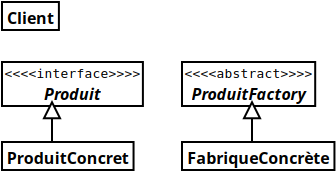
\includegraphics[width=.65\textwidth]{diagrammes/modele_generique_factory.png}
\caption{Modèle générique Factory}
\end{figure}

\end{document}
